% =============================================================================
%  Atto 3 — Gap analysis  (~10 min, ~6 slide)  [Parte I]
% =============================================================================

\section{The gap}

\begin{frame}{The gap, visualised}
  \centering
  \begin{tikzpicture}[node distance=8mm and 16mm]
    \node[hl]                  (nav)  {Nav2\\\scriptsize Controller~+~Smoother};
    \node[ghost, right=20mm of nav, minimum width=34mm, minimum height=22mm]
                                (gap)  {\Huge\textbf{?}};
    \node[ll, right=28mm of gap, minimum width=18mm]
                                (mot)  {4 motors\\\scriptsize PWM duty cycles};

    \draw[arrhl] (nav) -- node[above, msg]
      {\(v_x\), \(\omega_z\)} node[below, msg] {\texttt{TwistStamped}} (gap);
    \draw[arrgap] (gap) -- node[above, msg]
      {\(d_{FL}, d_{FR}, d_{RL}, d_{RR}\)} (mot);

    \node[layerlbl, above=1mm of nav] {high-level / soft real-time};
    \node[layerlbl, above=1mm of mot] {low-level / hard real-time};
    \node[font=\scriptsize\bfseries\itshape, text=Accent, below=1mm of gap]
      {what do we have to build?};
  \end{tikzpicture}

  \vspace{1.2em}
  \begin{itemize}\setlength\itemsep{2pt}
    \item \textbf{Left side:} an \emph{abstract} body-frame velocity, sampled at
          tens of Hz, on a ROS topic.
    \item \textbf{Right side:} four \emph{concrete} duty cycles that have to be
          regulated at \emph{hundreds} of Hz on bare metal.
    \item In between: \textbf{kinematics, control, transport, feedback,
          diagnostics, safety}.
  \end{itemize}
\end{frame}

% ---------------------------------------------------------------------------- %
\begin{frame}{Decomposing the gap}
  Five distinct functions sit between \texttt{cmd\_vel} and the H-bridge:

  \vspace{0.4em}
  \begin{enumerate}\setlength\itemsep{3pt}
    \item \textbf{Inverse kinematics.}\;
          Map \((v_x,\omega_z)\) to per-wheel angular references
          \(d_i\) using wheel radius \(r\) and track width \(b\):
          \[
            d_{\text{L}} = \frac{v_x-\tfrac{b}{2}\,\omega_z}{r},\quad
            d_{\text{R}} = \frac{v_x+\tfrac{b}{2}\,\omega_z}{r}
          \]
    \item \textbf{Wheel-level closed-loop control.}\;
          Track \(d_i\) with a per-motor regulator
          (e.g.\ PID + anti-windup) generating PWM.
    \item \textbf{Forward kinematics \& odometry.}\;
          Reconstruct \((v_x,\omega_z)\) — and integrate to a pose — from
          encoder feedback, publishing \texttt{nav\_msgs/Odometry} and
          the \texttt{odom}\(\to\)\texttt{base\_link} transform.
    \item \textbf{Transport \& contract.}\;
          Carry references \emph{down} and feedback \emph{up} across the
          companion-computer / MCU boundary on a deterministic bus.
    \item \textbf{Lifecycle \& fail-safe.}\;
          Bring-up order, watchdogs, zero-on-timeout, e-stop.
  \end{enumerate}
\end{frame}

% ---------------------------------------------------------------------------- %
\section{ros2\_control to the rescue}

\begin{frame}{ros2\_control in one slide}
  \begin{columns}[T,onlytextwidth]
    \column{0.45\textwidth}
      \textbf{Three moving parts.}
      \begin{itemize}\setlength\itemsep{4pt}
        \item \texttt{controller\_manager}: fixed-rate tick.
        \item Controllers: kinematics and odometry.
        \item \texttt{SystemInterface}: real hardware access.
      \end{itemize}

      \vspace{0.5em}
      \alert{Key split:}\\
      \emph{reusable controller} vs.\ \emph{custom hardware plugin}.

    \column{0.50\textwidth}
      \centering
      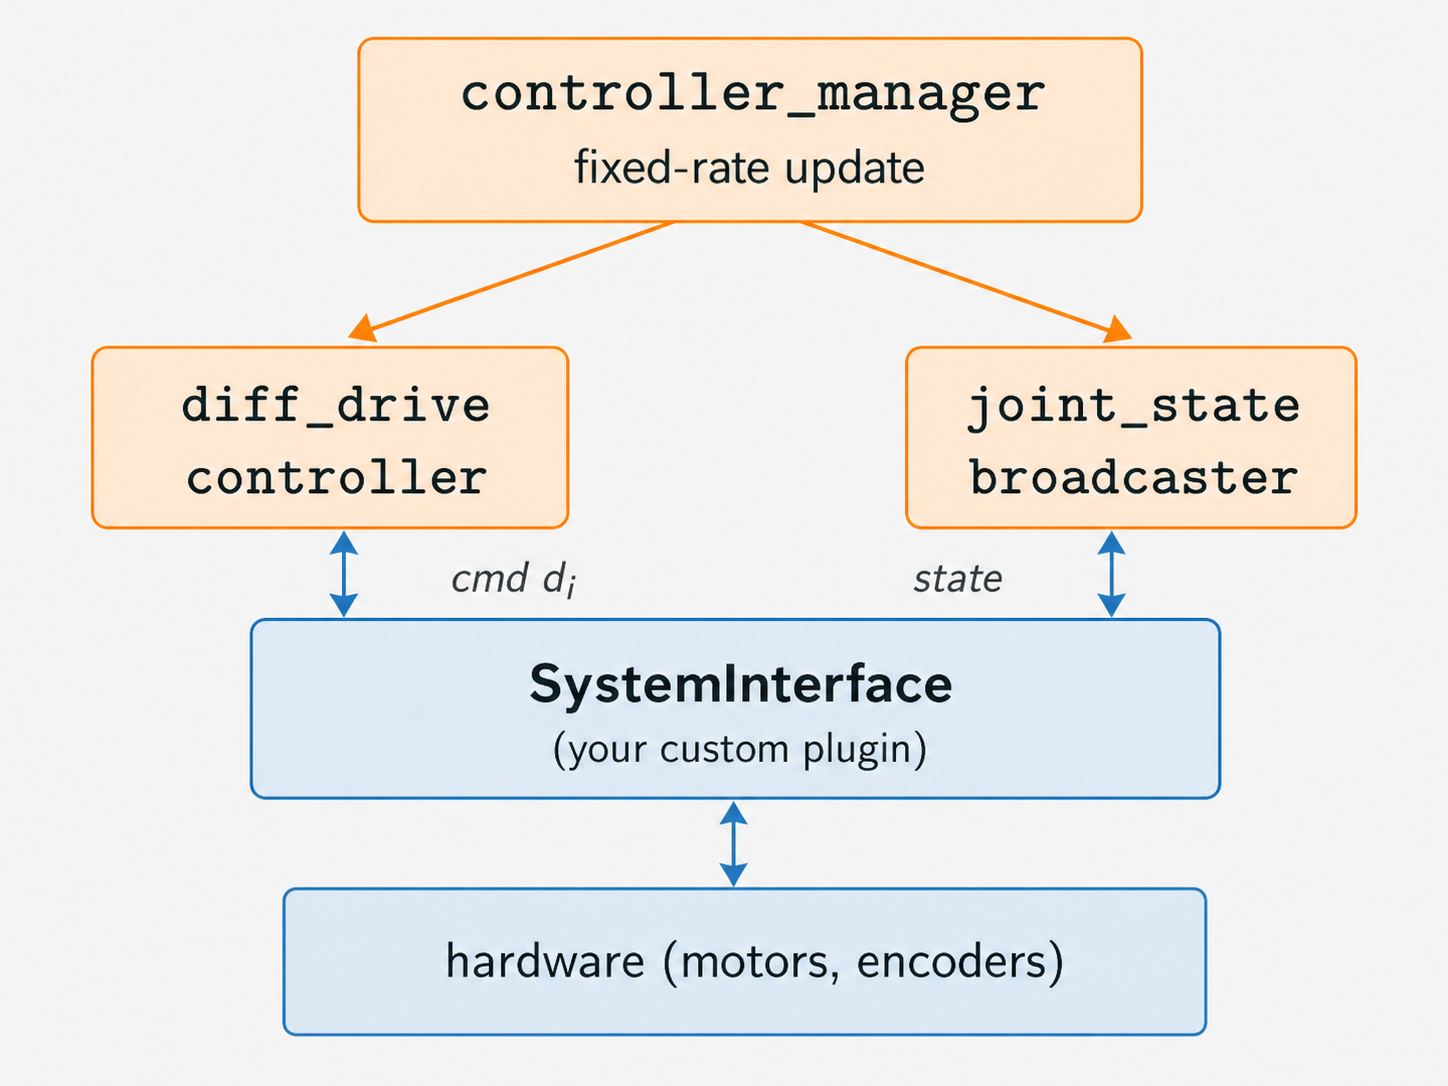
\includegraphics[width=\linewidth,height=0.62\textheight,keepaspectratio]{images/03_ros2_control_in_one_slide.png}
  \end{columns}
\end{frame}

% ---------------------------------------------------------------------------- %
\begin{frame}{Where ros2\_control plugs into the gap}
  \centering
  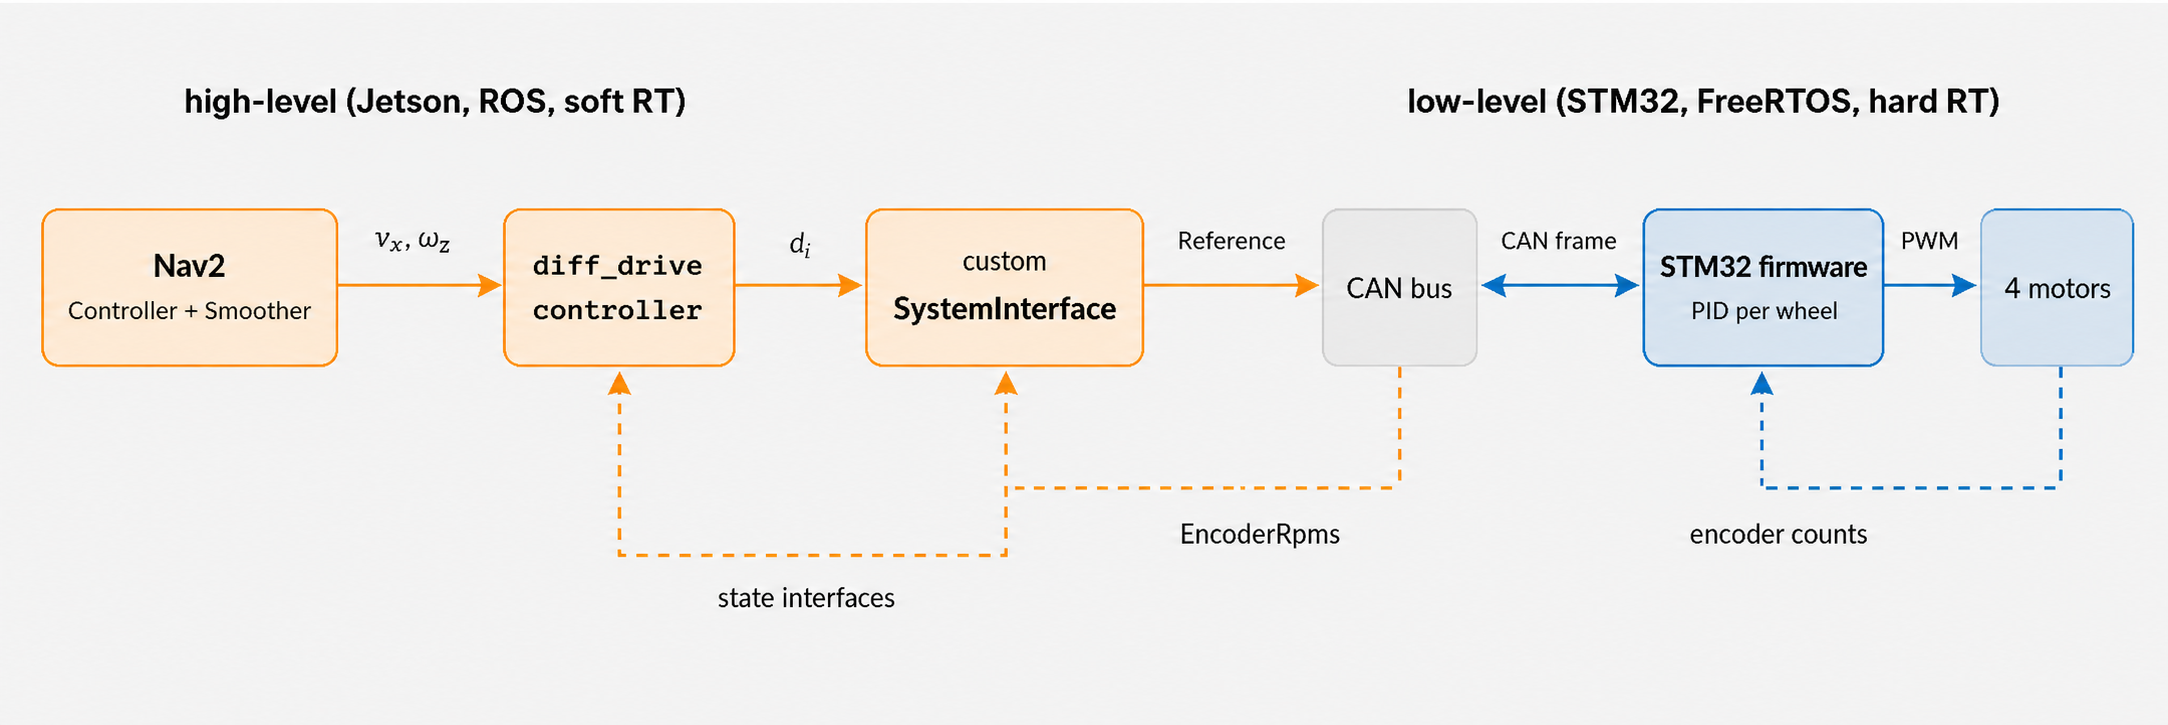
\includegraphics[width=0.98\textwidth,height=0.58\textheight,keepaspectratio]{images/03_ros2_control_plugs.png}

  \vspace{0.6em}
  \begin{itemize}\setlength\itemsep{2pt}
    \item \texttt{diff\_drive\_controller} solves the inverse \emph{and} the forward kinematics.
    \item Our \texttt{MiviaRoverSystem} is the \alert{only piece we have to write on the ROS side}.
    \item Everything to the right of the bus is the firmware's job.
  \end{itemize}
\end{frame}

% ---------------------------------------------------------------------------- %
\section{High-level vs.\ low-level: where to draw the line}

\begin{frame}{Two worlds, one contract}
  \centering
  \resizebox{\textwidth}{!}{%
  \begin{tikzpicture}
    \node[hl, text width=55mm, minimum height=26mm, align=left,
          inner xsep=4mm, inner ysep=3mm] (hlbox) {
      \scriptsize
      \textbullet\ Nav2: planning, BT, costmaps\\
      \textbullet\ \texttt{diff\_drive\_controller}:\\
      \hspace*{1.4em}kinematics + odometry\\
      \textbullet\ Custom \texttt{SystemInterface}:\\
      \hspace*{1.4em}ROS \(\leftrightarrow\) CAN\\
      \textbullet\ Localization, perception, mapping\\
      \textbullet\ Best-effort scheduling
    };

    \node[bus, minimum width=18mm, minimum height=17mm,
          right=7mm of hlbox] (bus)
      {CAN\\\scriptsize \texttt{1\,Mbit/s}\\\scriptsize \textbf{DBC}};

    \node[ll, text width=55mm, minimum height=26mm, align=left,
          inner xsep=4mm, inner ysep=3mm, right=7mm of bus] (llbox) {
      \scriptsize
      \textbullet\ Encoder acquisition\\
      \textbullet\ Per-wheel PID at \(200\)~Hz, anti-windup\\
      \textbullet\ PWM generation, H-bridge driving\\
      \textbullet\ CAN ISR + service task\\
      \textbullet\ Watchdog, fail-stop, no \texttt{malloc}\\
      \textbullet\ Hard real-time deterministic scheduling
    };

    \node[layerlbl, above=1mm of hlbox]
      {High-level — Jetson, ROS~2, soft real-time};
    \node[layerlbl, above=1mm of llbox]
      {Low-level — STM32F7, FreeRTOS, hard real-time};

    \draw[arr, <->, line width=0.7pt] (hlbox.east) -- (bus.west);
    \draw[arr, <->, line width=0.7pt] (bus.east) -- (llbox.west);
  \end{tikzpicture}}

  \vspace{0.4em}
  \footnotesize
  The two layers are decoupled by an \textbf{explicit, versionable communication
  contract} (the \texttt{.dbc} file) — software and firmware evolve
  independently as long as the contract is preserved.
\end{frame}

% ---------------------------------------------------------------------------- %
\begin{frame}{Why split here, and not somewhere else?}
  \begin{columns}[T,onlytextwidth]
    \column{0.50\textwidth}
      \textbf{Things that \emph{must} live near the silicon.}
      \begin{itemize}\setlength\itemsep{2pt}
        \item Tight, jitter-free timing (PWM, encoder reads).
        \item Saturation, anti-windup, motor-side safety.
        \item Behaviour under loss of communication.
      \end{itemize}

      \textbf{Things that \emph{want} to live in ROS.}
      \begin{itemize}\setlength\itemsep{2pt}
        \item Map / costmap reasoning, BT, planners.
        \item Multi-modal sensing fusion, learning modules.
        \item Anything that benefits from a Linux userspace.
      \end{itemize}

    \column{0.50\textwidth}
      \textbf{Drawing the line at \emph{wheel-velocity references}:}
      \begin{itemize}\setlength\itemsep{2pt}
        \item \alert{High-level} delivers a setpoint \(d_i\)
              and \emph{trusts} the firmware to track it.
        \item \alert{Low-level} reports a measurement
              \(\hat{d}_i\) and \emph{trusts} the host to do the
              kinematics.
        \item Asymmetries between motors / encoders / chains are absorbed at
              the wheel level — they never leak into Nav2.
      \end{itemize}

      \vspace{0.4em}
      \footnotesize\textcolor{black!60}{This is the same boundary used in
      most production AGV / AMR stacks: speed setpoints across the bus,
      kinematics and odometry on the host.}
  \end{columns}
\end{frame}

% ---------------------------------------------------------------------------- %
\section{What we have established}

\begin{frame}{Take-aways from Part~I}
  \begin{enumerate}\setlength\itemsep{4pt}
    \item Nav2's chain ends at the \textbf{Velocity Smoother}, whose only
          deliverable is a single \texttt{TwistStamped} on \texttt{cmd\_vel}
          --- two scalars for a differential-drive robot.
    \item A custom 4-motor platform speaks an entirely different language:
          per-wheel \textbf{PWM duty cycles} regulated in hard real-time.
    \item The gap consists of \textbf{five concrete responsibilities}:
          inverse kinematics, wheel-level control, odometry, transport,
          and lifecycle/safety.
    \item \textbf{ros2\_control} factorises that gap into a reusable
          controller (\texttt{diff\_drive\_controller}) and a
          hardware-specific plugin (your \texttt{SystemInterface}).
    \item The \emph{natural place to split} ROS from firmware is the
          \textbf{wheel-velocity reference}: kinematics on the host,
          regulation on the MCU, an explicit \textbf{DBC contract} on the
          bus.
  \end{enumerate}
\end{frame}

% ---------------------------------------------------------------------------- %
\begin{frame}{Coming next — the recipe (Part~II)}
  Now that we know \emph{what} is missing, we will look at \emph{how} to
  build it on the MiviaRover, in three subparts:
  \vspace{0.6em}

  \begin{columns}[T,onlytextwidth]
    \column{0.33\textwidth}
      \textbf{II.A — Downstream}\\
      \footnotesize\textcolor{black!60}{\(v_x,\omega_z\) $\to$ wheels}
      \begin{enumerate}\setlength\itemsep{2pt}
        \item URDF/xacro \(+\) \texttt{<ros2\_control>}
        \item Controllers YAML
        \item Custom \texttt{MiviaRoverSystem}
        \item ROS-side CAN stack
        \item Bring-up order
      \end{enumerate}

    \column{0.33\textwidth}
      \textbf{II.B — Upstream \& contract}\\
      \footnotesize\textcolor{black!60}{Encoders $\to$ \texttt{/odom}}
      \begin{enumerate}\setlength\itemsep{2pt}
        \item Firmware tx of RPMs
        \item \texttt{report\_parser}
        \item \texttt{read()} \(+\) watchdog
        \item Forward kinematics
        \item DBC contract pattern
      \end{enumerate}

    \column{0.33\textwidth}
      \textbf{II.C — Firmware}\\
      \footnotesize\textcolor{black!60}{Bare-metal RT loop}
      \begin{enumerate}\setlength\itemsep{2pt}
        \item Why an MCU at all
        \item Bring-up sequence
        \item Inner loop @ \(200\)~Hz
        \item Tasks \& schedulability
        \item Fail handling
      \end{enumerate}
  \end{columns}

  \vspace{1.0em}
  \centering
  \alert{\textit{End of Part~I — questions on the gap before we open the recipe?}}
\end{frame}
